\documentclass[11pt,a4paper]{article}

% ── packages ─────────────────────────────────────────────────────
\usepackage[margin=25mm]{geometry}
\usepackage{amsmath,amssymb}
\usepackage{graphicx}
\usepackage{booktabs}
\usepackage{hyperref}
\usepackage{xcolor}
\usepackage{float}
\usepackage{caption}
\usepackage{subcaption}

\hypersetup{colorlinks=true, linkcolor=blue!60!black, citecolor=green!50!black, urlcolor=blue!70!black}

\graphicspath{{figures/}}

% ── custom commands ──────────────────────────────────────────────
\newcommand{\phimax}{\phi_{\mathrm{max}}}
\newcommand{\thetamax}{\theta_{\mathrm{max}}}
\newcommand{\pvz}{z_{\mathrm{PV}}}
\newcommand{\zcrit}{z_{\mathrm{crit}}}
\newcommand{\halfx}{L_x}

% ─────────────────────────────────────────────────────────────────
\title{Segment-Grass Effect:\\
       Anomalous Occupancy Sub-peaks at \boldmath$\pm 0.2$\,rad\\[4pt]
       \large A Geometric Clipping Artefact in the Toy VELO Model}
\author{G.\ Scriven}
\date{\today}

\begin{document}
\maketitle

% =================================================================
\begin{abstract}
The hit-occupancy histograms produced by the \texttt{hit\_competition\_study}
notebook exhibit small but persistent sub-peaks (``segment grass'') that
appear \emph{only} at the $\pm 0.2$\,rad angle setting and are absent at
$\pm 0.1$ and $\pm 0.04$\,rad.  This note traces the effect to its root
cause: \textbf{geometric clipping} of extreme-angle tracks on the outermost
detector modules when the primary vertex is generated far upstream of the
detector.  We quantify the clipping probability analytically, confirm it
with Monte Carlo, and show the direct track-level correspondence between
clipped tracks and anomalous occupancy values.
\end{abstract}

% =================================================================
\section{Introduction}
\label{sec:intro}

In the toy VELO tracking model, candidate segments are constructed between
every pair of hits on adjacent detector modules.  The \emph{hit occupancy}
--- the number of candidate segments using a given hit --- is a key
diagnostic.  For an event with $n$ tracks per module, a hit on an internal
module connects to hits on both neighbours, giving an expected occupancy of
$\sim 2n$.  Hits on the first or last module connect to one neighbour only,
so their expected occupancy is~$n$.

The \texttt{hit\_competition\_study} notebook revealed that at the
$\pm 0.2$\,rad generation angle setting, the occupancy histograms contain
small spikes at values below the expected $n$ and $2n$ peaks.  These
``grass'' features are completely absent at the narrower $\pm 0.1$ and
$\pm 0.04$\,rad settings.  This note investigates the origin of these
anomalies.

% =================================================================
\section{Geometry and Generation Parameters}
\label{sec:geometry}

The toy detector consists of $N_{\text{mod}} = 5$ planar modules at
$z$-positions:
\begin{equation}
  z_k = 100 + 33k \quad \text{mm}, \qquad k = 0, 1, \ldots, 4,
\end{equation}
each with half-width $\halfx = 50$\,mm in both $x$ and $y$.

Particles originate from a primary vertex (PV) whose coordinates are
sampled from
\begin{equation}
  \pvz \sim \mathcal{N}(0,\, \sigma_z^2), \qquad \sigma_z = 50\,\text{mm}.
\end{equation}
Crucially, this sampling is performed \textbf{independently for every
generated event}.  In the \texttt{hit\_competition\_study} notebook, the
call
\begin{verbatim}
  gen.generate_random_primary_vertices({"x": 0.1, "y": 0.1, "z": 50.0})
\end{verbatim}
is made inside the per-event loop, so each event in the density sweep
draws a fresh PV position.  The argument \texttt{"z": 50.0} specifies
$\sigma_z = 50$\,mm (not a fixed PV position).  As a result, the PV
$z$-coordinate varies substantially across the ensemble: roughly 68\,\% of
events have $\pvz \in [-50, +50]$\,mm, but the tails extend far upstream.
In particular, $\sim$38\,\% of events have $\pvz < -14.7$\,mm --- the
critical threshold for module-4 clipping at $\pm 0.2$\,rad (see
Section~\ref{sec:rootcause}).  This event-by-event variation in PV
position is the direct cause of the variable number of clipped tracks and,
consequently, the spread of anomalous occupancy values (``segment grass'')
in the histograms.

Track angles (slopes) are sampled uniformly:
\begin{equation}
  \phi \sim \mathcal{U}(-\phimax,\, +\phimax), \qquad
  t_x = \tan\phi, \qquad
  \text{(analogously for } \theta, t_y\text{)}.
\end{equation}

% =================================================================
\section{Root Cause: Geometric Clipping}
\label{sec:rootcause}

A particle with slope $t_x = \tan\phimax$ originating at $\pvz$ reaches
transverse position
\begin{equation}
  x(z_k) = x_{\mathrm{PV}} + t_x (z_k - \pvz)
  \label{eq:xpos}
\end{equation}
at module~$k$.  The hit is recorded only if $|x| \le \halfx$.  The maximum
displacement occurs at the last module and at the largest angle.  The
critical PV $z$-position beyond which a track at $\phi = \phimax$ misses
module~$k$ is
\begin{equation}
  \boxed{\;
    \zcrit^{(k)} = z_k - \frac{\halfx}{\tan\phimax}
  \;}
  \label{eq:zcrit}
\end{equation}
For $\phimax = 0.2$\,rad ($\tan 0.2 \approx 0.203$), the critical values
and associated clipping probabilities
$P_{\text{clip}} = \Phi\!\bigl((\zcrit - 0)/\sigma_z\bigr)$
are listed in Table~\ref{tab:clipping}.

\begin{table}[H]
  \centering
  \caption{Critical PV $z$-positions and clipping probabilities for each
           module at $\phimax = 0.2$\,rad.}
  \label{tab:clipping}
    \begin{tabular}{@{}cccc@{}}
    \toprule
    Module $k$ & $z_k$ (mm) & $\zcrit^{(k)}$ (mm) & $P_{\text{clip}}$ (\%) \\
    \midrule
    0 & 100 & $-146.7$ &  0.2 \\
    1 & 133 & $-113.7$ &  1.2 \\
    2 & 166 & $ -80.7$ &  5.3 \\
    3 & 199 & $ -47.7$ & 17.0 \\
    4 & 232 & $ -14.7$ & 38.5 \\
    \bottomrule
  \end{tabular}
\end{table}

For the narrower angle settings:
\begin{itemize}
  \item $\phimax = 0.1$\,rad: $\zcrit^{(4)} \approx -266$\,mm
        ($> 5\sigma$, probability $< 10^{-5}\%$).
  \item $\phimax = 0.04$\,rad: $\zcrit^{(4)} \approx -1019$\,mm
        (effectively impossible).
\end{itemize}
This explains why the effect is observed \emph{only} at $\pm 0.2$\,rad.

Figure~\ref{fig:clipping_probability} illustrates the PV $z$ distribution
overlaid with the module clipping thresholds.

\begin{figure}[H]
  \centering
  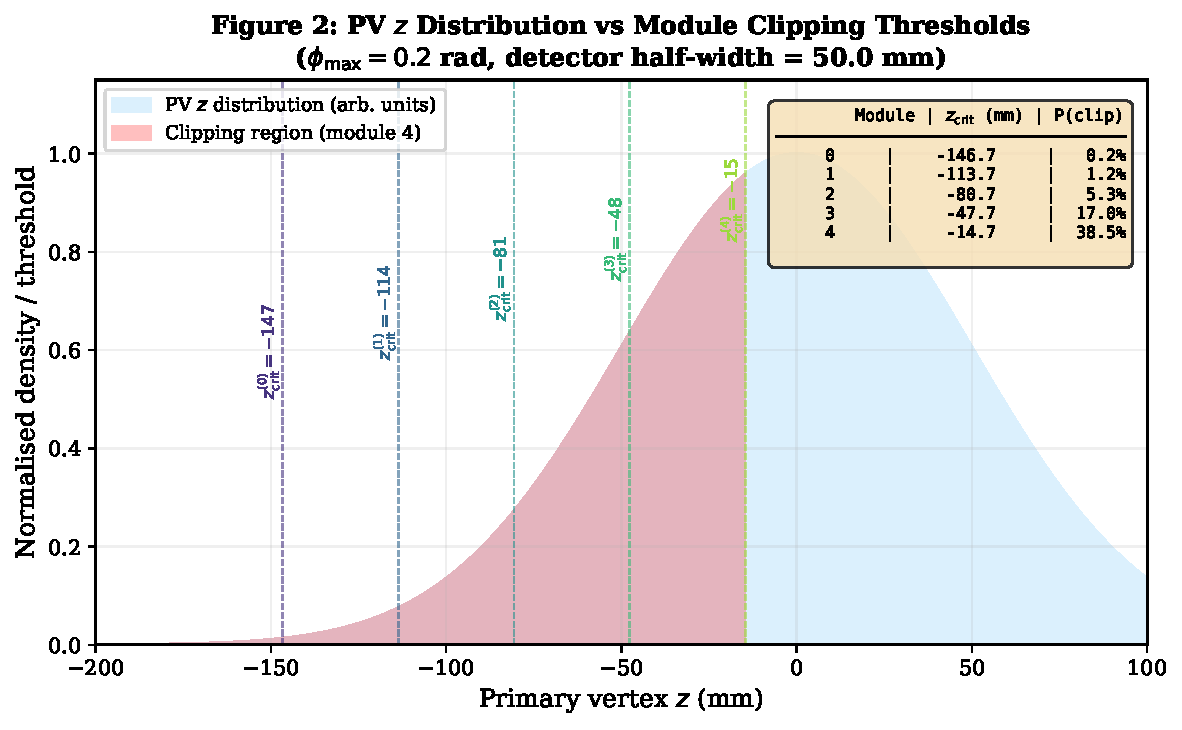
\includegraphics[width=0.85\textwidth]{fig2_clipping_probability}
  \caption{PV $z$ distribution (blue shading) with clipping thresholds
           for each module (vertical dashed lines).  The red-shaded region
           shows PV positions that cause at least one track to miss
           module~4.}
  \label{fig:clipping_probability}
\end{figure}

% =================================================================
\section{Mechanism: How Clipping Creates Occupancy Sub-peaks}
\label{sec:mechanism}

The segment construction creates all $n_i \times n_{i+1}$ segments between
adjacent modules $i$ and $i{+}1$, where $n_i$ is the hit count on
module~$i$.  For a hit on module~$k$ (internal), the occupancy is:
\begin{equation}
  \text{occ}(k) = n_{k-1} + n_{k+1}.
\end{equation}

When all tracks are accepted, $n_k = n_{\text{tracks}}$ for every module,
giving the expected occupancy of $2n_{\text{tracks}}$.

However, when some extreme-angle tracks miss module~4, the hit count on
that module drops: $n_4 < n_{\text{tracks}}$.  This directly reduces the
occupancy of every hit on module~3:
\begin{equation}
  \text{occ}(3) = n_2 + n_4 = n_{\text{tracks}} + n_4 < 2n_{\text{tracks}}.
\end{equation}

Since the number of clipped tracks varies event-by-event (depending on the
PV $z$ position and the specific random angles), $n_4$ takes a range of
values across the ensemble, producing a spread of occupancy values below
the expected peak.  These are the ``grass'' sub-peaks in the histograms.

% =================================================================
\section{Direct Evidence}
\label{sec:evidence}

% ── 5.1 event displays ──────────────────────────────────────────
\subsection{Event Displays}

Figure~\ref{fig:event_displays} compares two events: one with the PV close to
the detector (no clipping) and one with the PV far upstream (multiple
clipped tracks shown in red).

\begin{figure}[H]
  \centering
  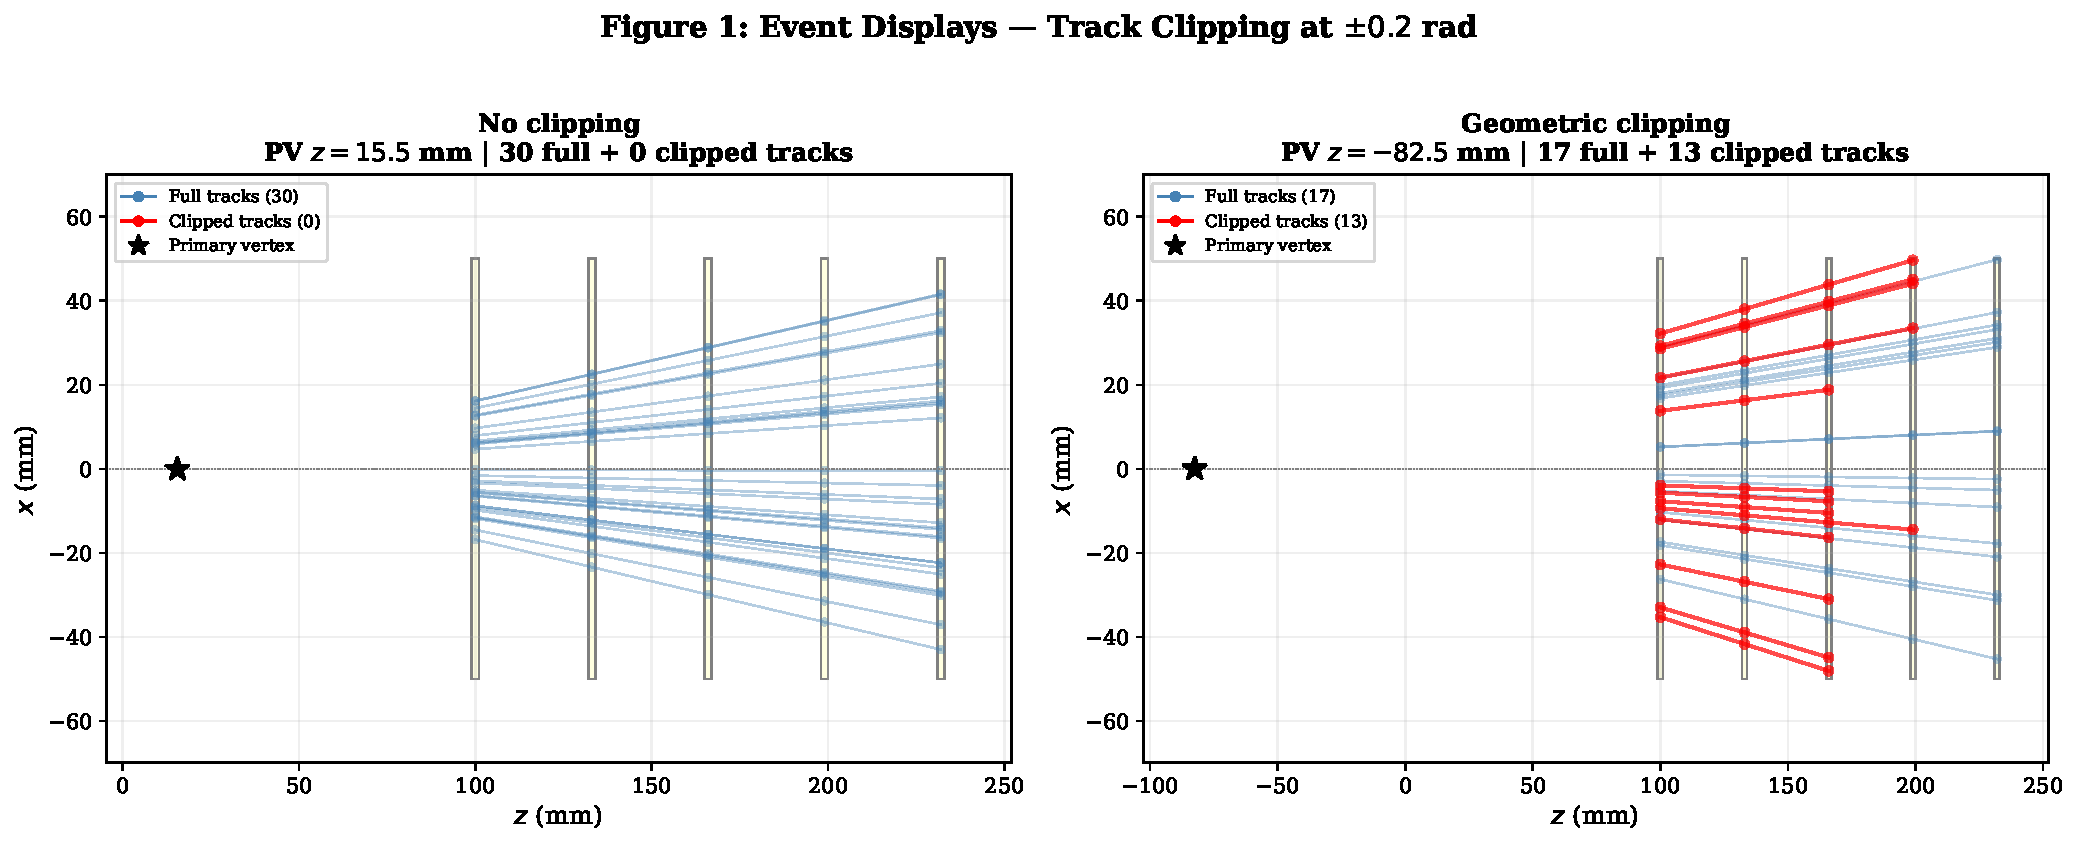
\includegraphics[width=\textwidth]{fig1_event_displays}
  \caption{Event displays for a clean event (left) and a clipped event
           (right).  Red tracks miss one or more modules.  The gray dashed
           lines indicate the detector edge at $\pm 50$\,mm.}
  \label{fig:event_displays}
\end{figure}

% ── 5.2 track-level diagnosis ───────────────────────────────────
\subsection{Track-Level Diagnosis}

Figure~\ref{fig:track_diagnosis} presents a complete diagnosis for a single
event with clipping:
\begin{itemize}
  \item[(a)] Event display with clipped tracks (red) and their extrapolated
             miss positions ($\times$~markers beyond the detector edge).
  \item[(b)] The $(\phi, \theta)$ distribution of all tracks.  Clipped
             tracks (triangles) cluster near the angular boundaries at
             $|\phi| \approx 0.2$ or $|\theta| \approx 0.2$.
  \item[(c)] Box plot of per-module occupancy.  Module~3's occupancy dips
             below the expected $2n$ because module~4 has fewer hits.
  \item[(d)] Overall occupancy histogram for this event.  Red bins mark
             the anomalous values arising from clipping; each one can be
             traced directly to the reduced $n_4$ count.
\end{itemize}

\begin{figure}[H]
  \centering
  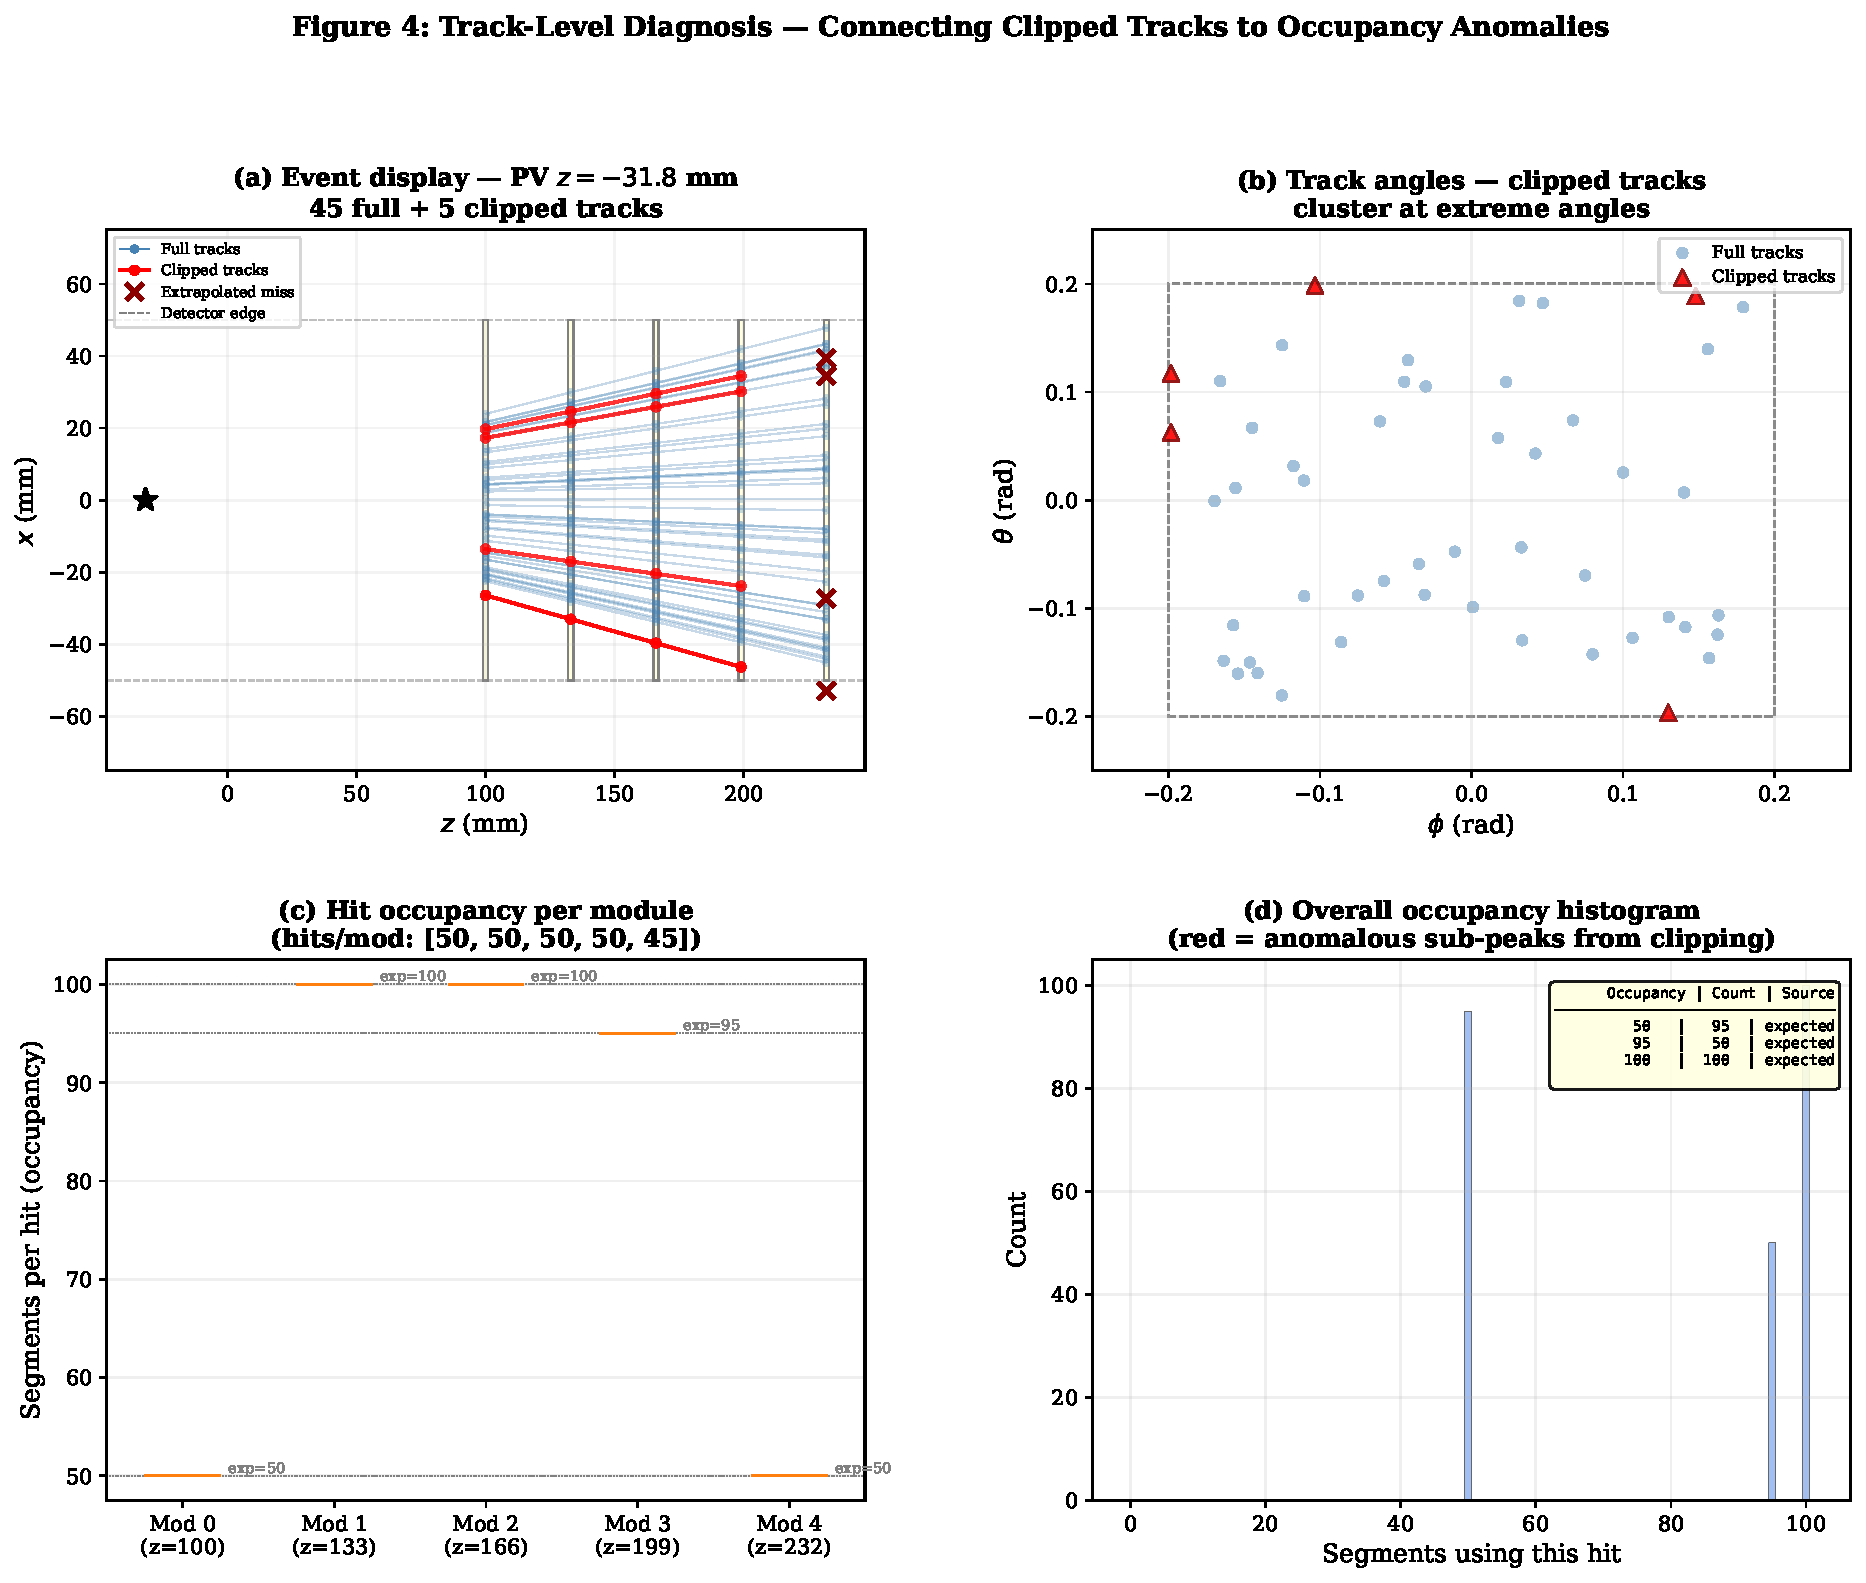
\includegraphics[width=\textwidth]{fig4_track_diagnosis}
  \caption{Complete track-level diagnosis.  (a)~Event display.
           (b)~Track angles --- clipped tracks (red triangles) lie near
           the $\pm 0.2$\,rad boundaries.
           (c)~Per-module occupancy box plots.
           (d)~Overall occupancy histogram with anomalous bins in red.}
  \label{fig:track_diagnosis}
\end{figure}

% ── 5.3 occupancy vs PV z ──────────────────────────────────────
\subsection{Occupancy vs Primary Vertex Position}

Figure~\ref{fig:occ_vs_pvz} shows the mean module-3 occupancy as a function of
PV $z$ across 200~events.  The occupancy is constant at the expected value
of $2n$ for $\pvz > \zcrit^{(4)}$ and decreases monotonically for more
negative PV positions, confirming the geometric origin.

\begin{figure}[H]
  \centering
  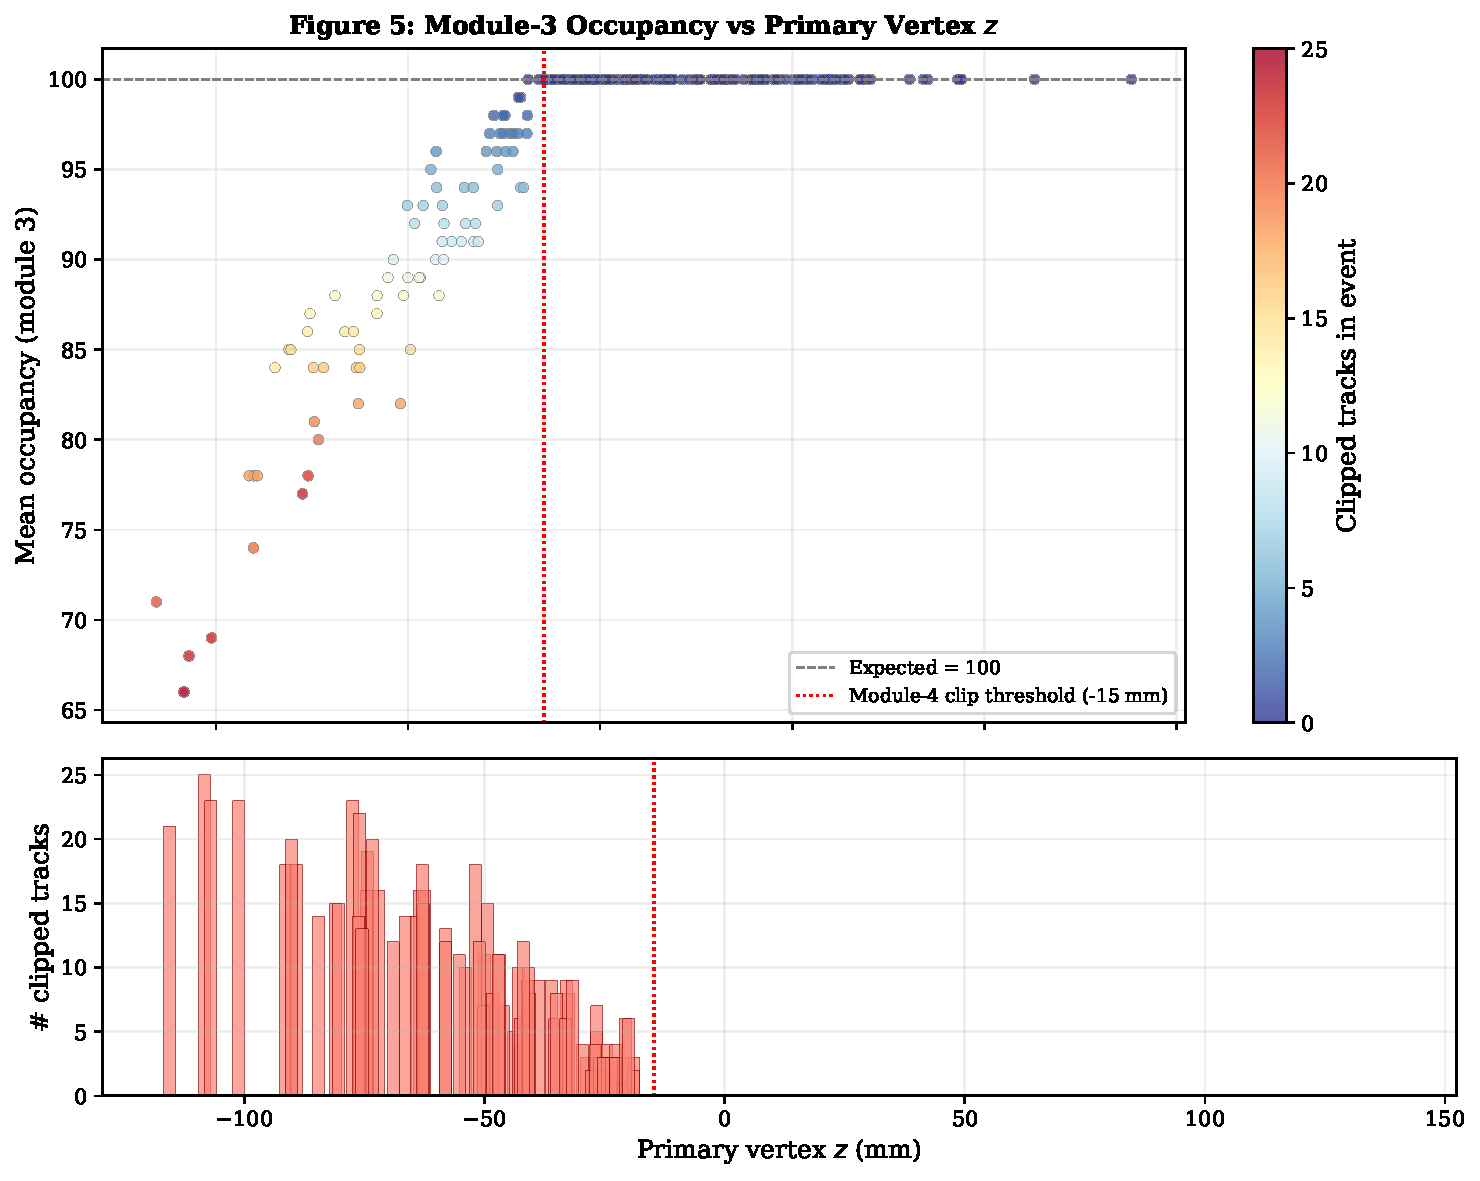
\includegraphics[width=0.85\textwidth]{fig5_occupancy_vs_pvz}
  \caption{Module-3 mean occupancy (top) and number of clipped tracks
           (bottom) vs PV $z$ position.  Points are coloured by the number
           of clipped tracks.  The red dotted line marks
           $\zcrit^{(4)} = -14.7$\,mm.}
  \label{fig:occ_vs_pvz}
\end{figure}

% ── 5.4 angle comparison ───────────────────────────────────────
\subsection{Angle-Setting Comparison}

Figure~\ref{fig:occ_comparison} compares the occupancy histograms for all three
angle settings ($\pm 0.2$, $\pm 0.1$, $\pm 0.04$\,rad) with 50~tracks per
event.  Anomalous sub-peaks (red) appear only in the $\pm 0.2$\,rad
setting.

\begin{figure}[H]
  \centering
  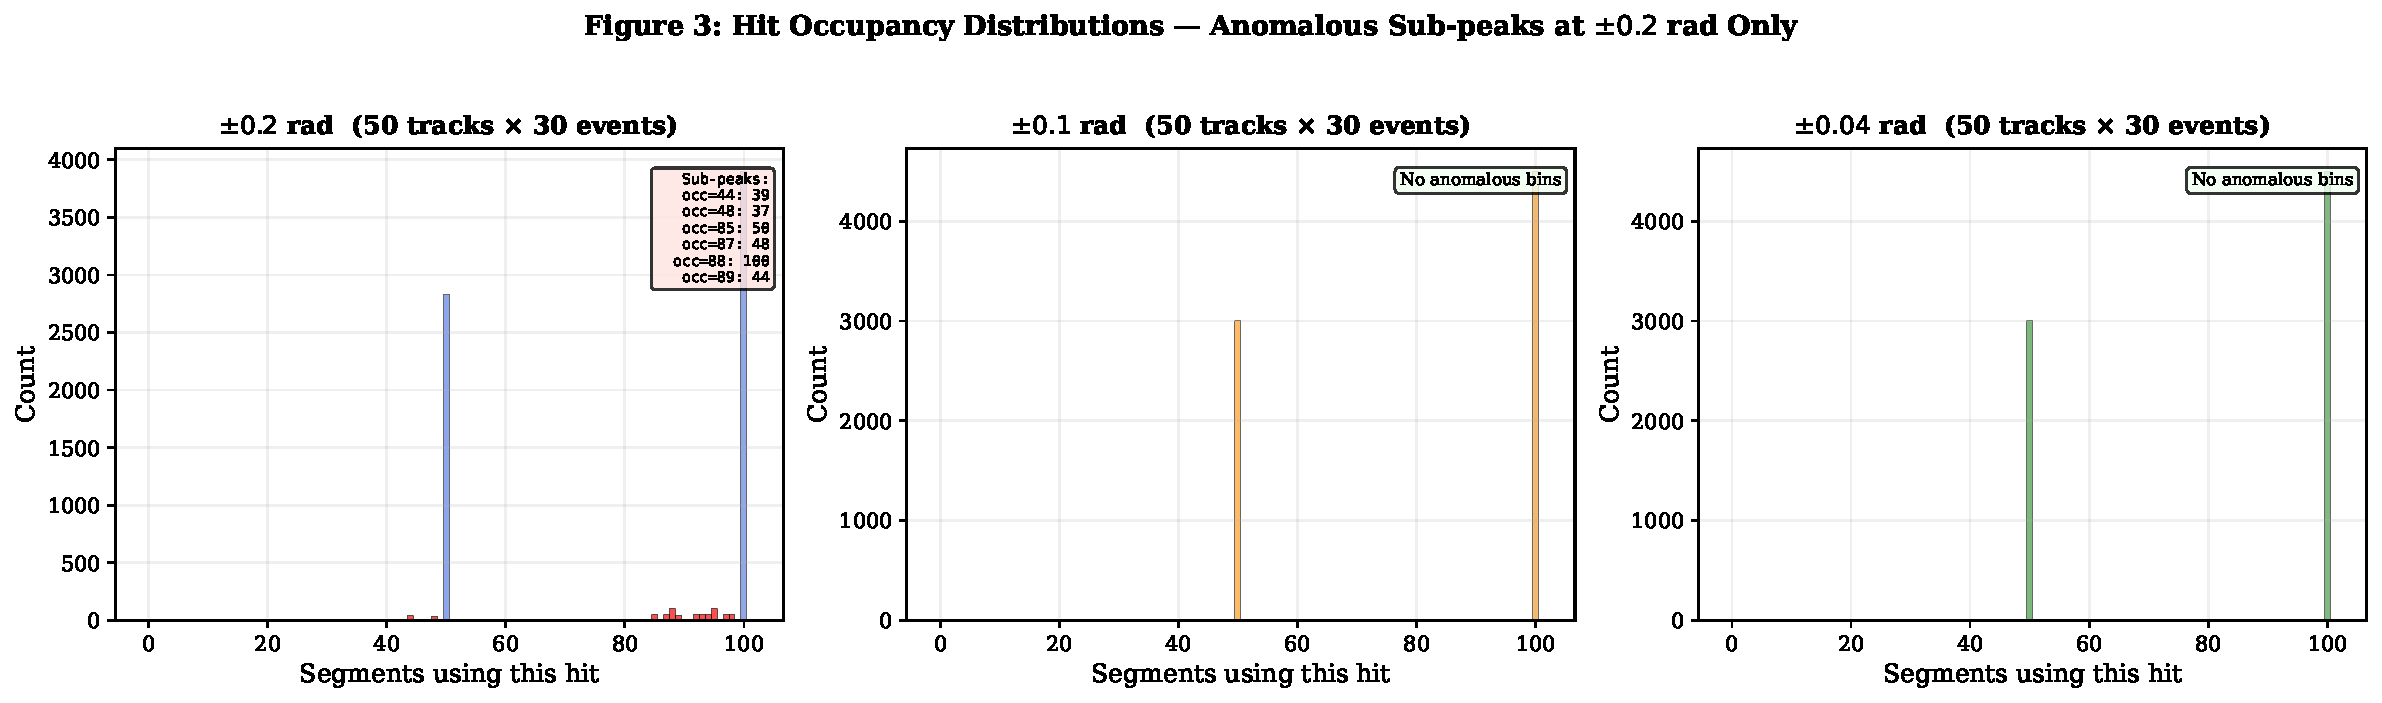
\includegraphics[width=\textwidth]{fig3_occupancy_comparison}
  \caption{Occupancy histograms for three angle settings.  Red bins
           indicate anomalous values absent from the expected peaks.
           Only the $\pm 0.2$\,rad setting exhibits sub-peaks.}
  \label{fig:occ_comparison}
\end{figure}

\subsection{Module Hit-Count Variability}

Figure~\ref{fig:hits_per_module} confirms that the per-module hit counts are
strictly constant at $n_{\text{tracks}}$ for the narrower angle settings,
but fluctuate on modules~3 and~4 at $\pm 0.2$\,rad.

\begin{figure}[H]
  \centering
  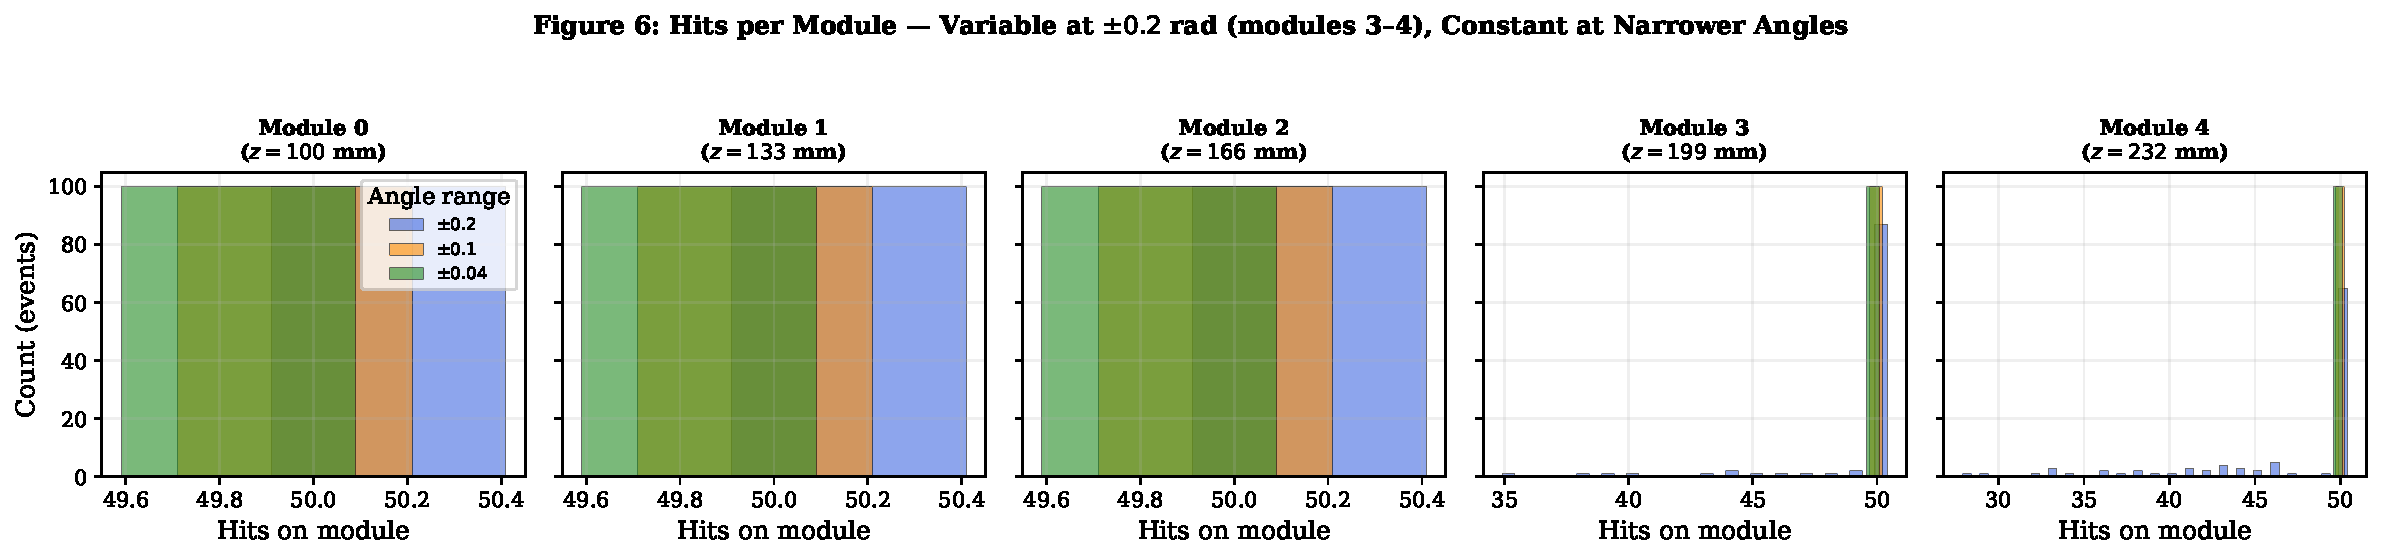
\includegraphics[width=\textwidth]{fig6_hits_per_module}
  \caption{Distribution of hits per module across 100~events for each
           angle setting.  At $\pm 0.2$\,rad (blue), modules~3 and~4 show
           variable hit counts due to geometric clipping.}
  \label{fig:hits_per_module}
\end{figure}

% =================================================================
\section{Systematic Sweep: Ghost Rate and Drop Rate}
\label{sec:sweep}

To understand how measurement noise interacts with the geometric clipping
effect, we perform a systematic sweep over two noise parameters:
\emph{ghost rate} (fraction of spurious hits added uniformly within module
bounds) and \emph{drop rate} (fraction of true hits randomly removed).  The
sweep covers a $6 \times 6$ grid:
ghost rate $\in \{0, 5, 10, 15, 20, 30\}\%$ and
drop rate $\in \{0, 5, 10, 15, 20, 30\}\%$, at two angle settings
($\pm 0.2$ and $\pm 0.1$\,rad) and three track multiplicities ($n = 20,
50, 100$), giving $216$ independent parameter points.  Each point averages
over 10 events.  The sweep was executed on HTCondor.

\subsection{Occupancy Histograms Under Noise}

Figure~\ref{fig:occ_clean} reproduces the original hit-competition
histograms from the clean baseline (ghost\,=\,0, drop\,=\,0), showing the
segment-grass sub-peaks at $\pm 0.2$\,rad and their absence at
$\pm 0.1$\,rad.  Figure~\ref{fig:occ_noisy} overlays several noisy
configurations on the same axes, demonstrating how ghost hits broaden the
distribution (shifting counts rightward) while dropped hits erode the
dominant peaks.

\begin{figure}[H]
  \centering
  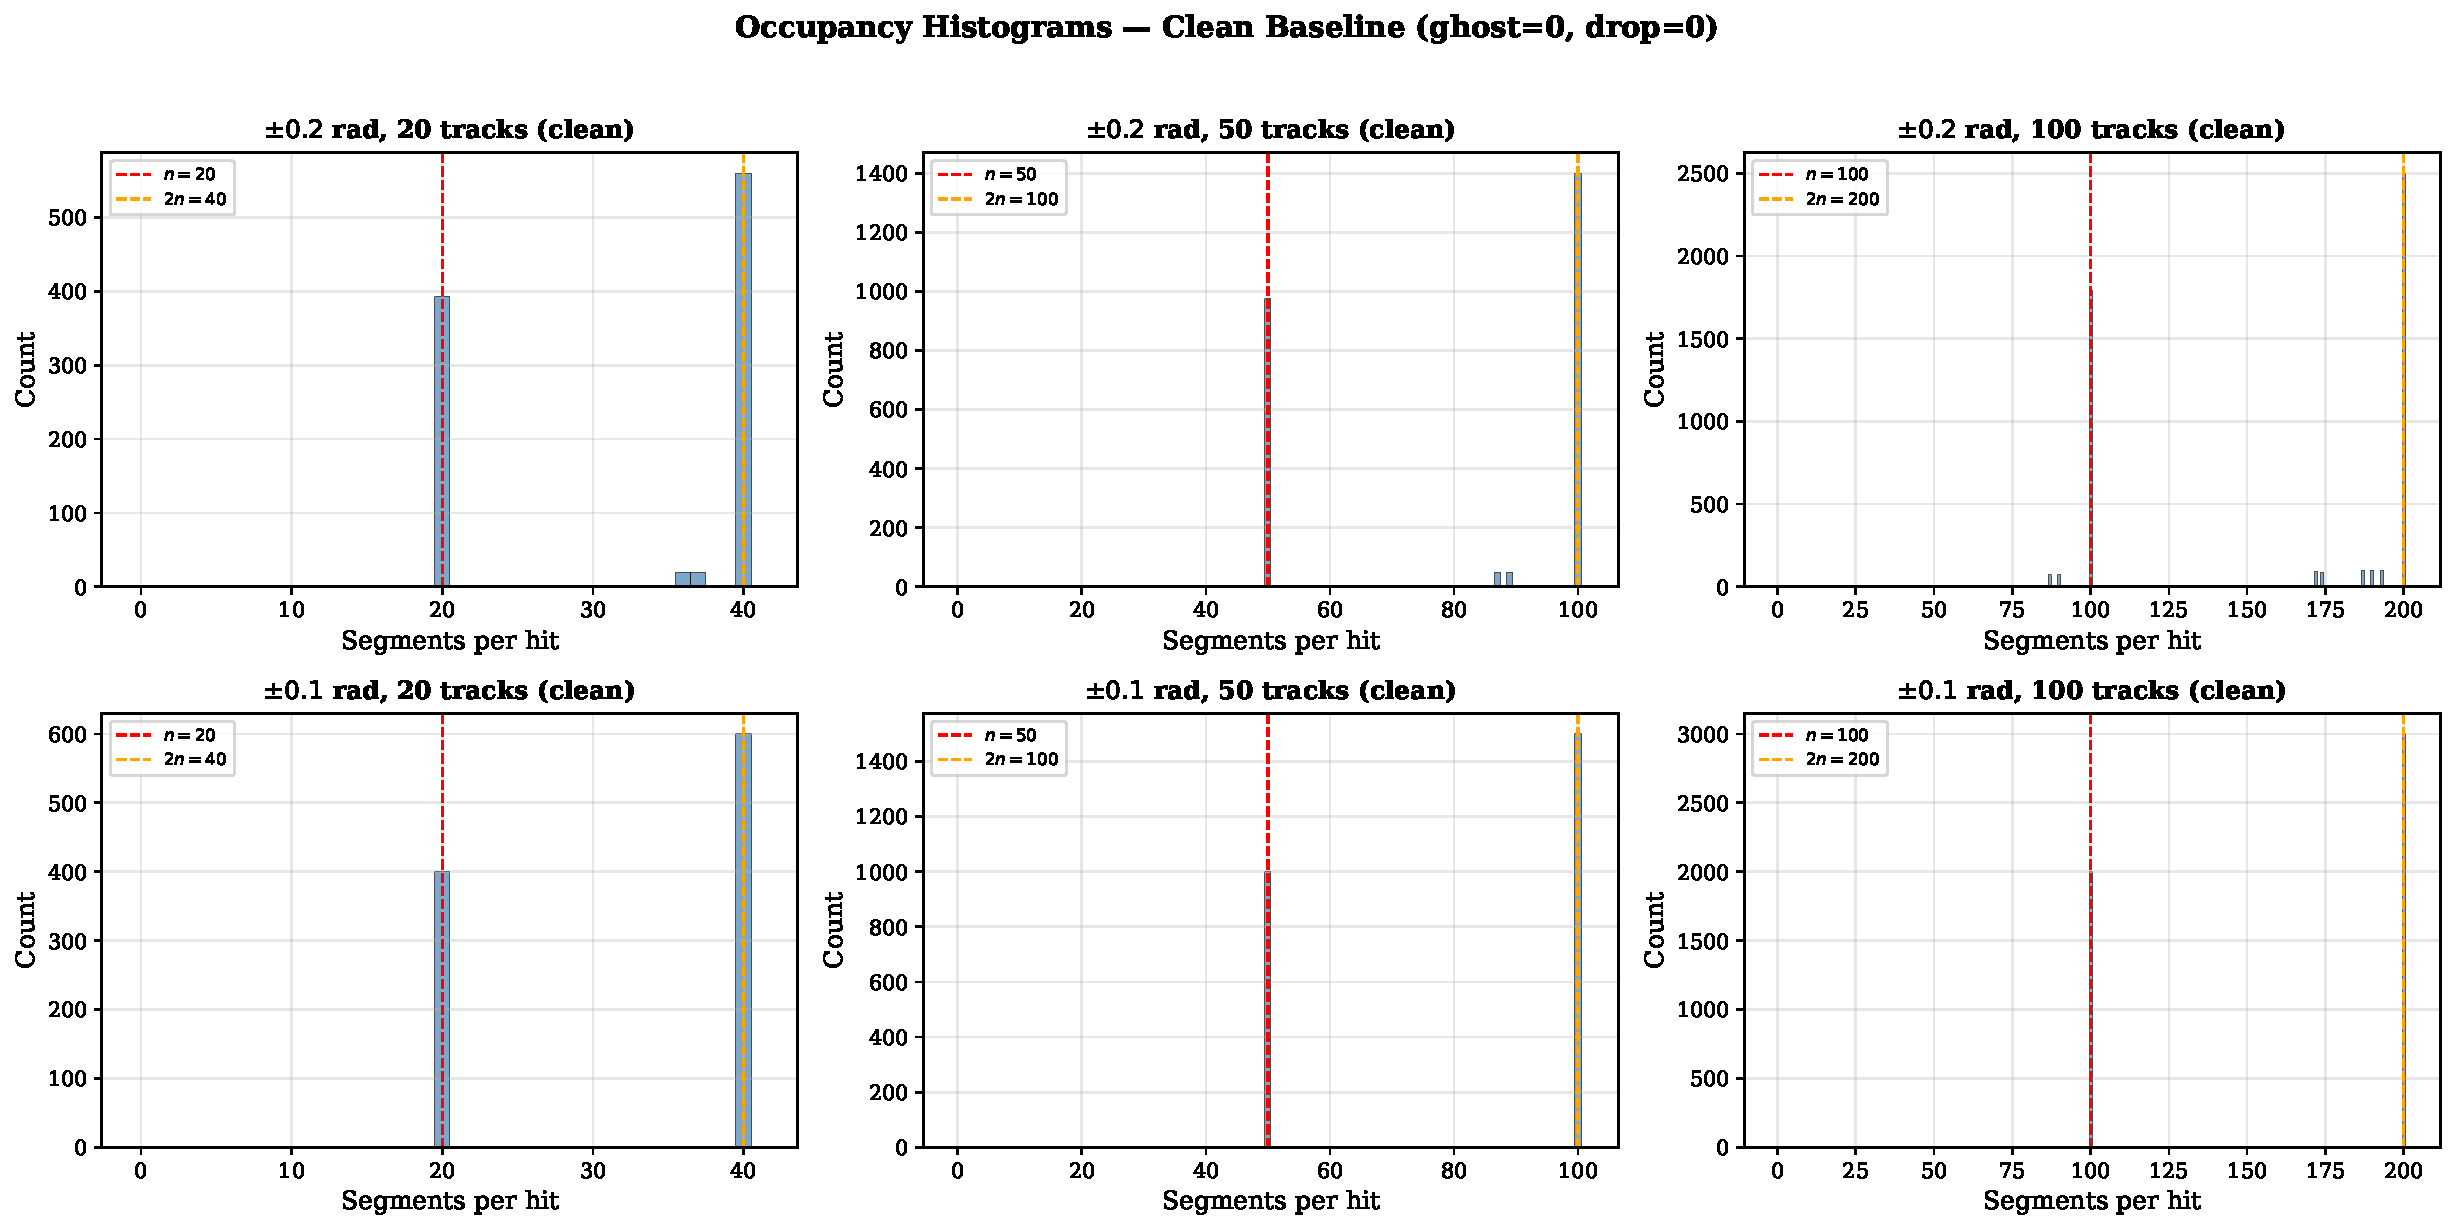
\includegraphics[width=\textwidth]{occ_hist_clean}
  \caption{Clean-baseline occupancy histograms ($2 \times 3$ grid: rows =
           angle settings, columns = track counts).  Dashed lines mark
           the expected $n$ and $2n$ peaks.  Sub-peaks visible at
           $\pm 0.2$\,rad (top row) are the segment-grass artefact.}
  \label{fig:occ_clean}
\end{figure}

\begin{figure}[H]
  \centering
  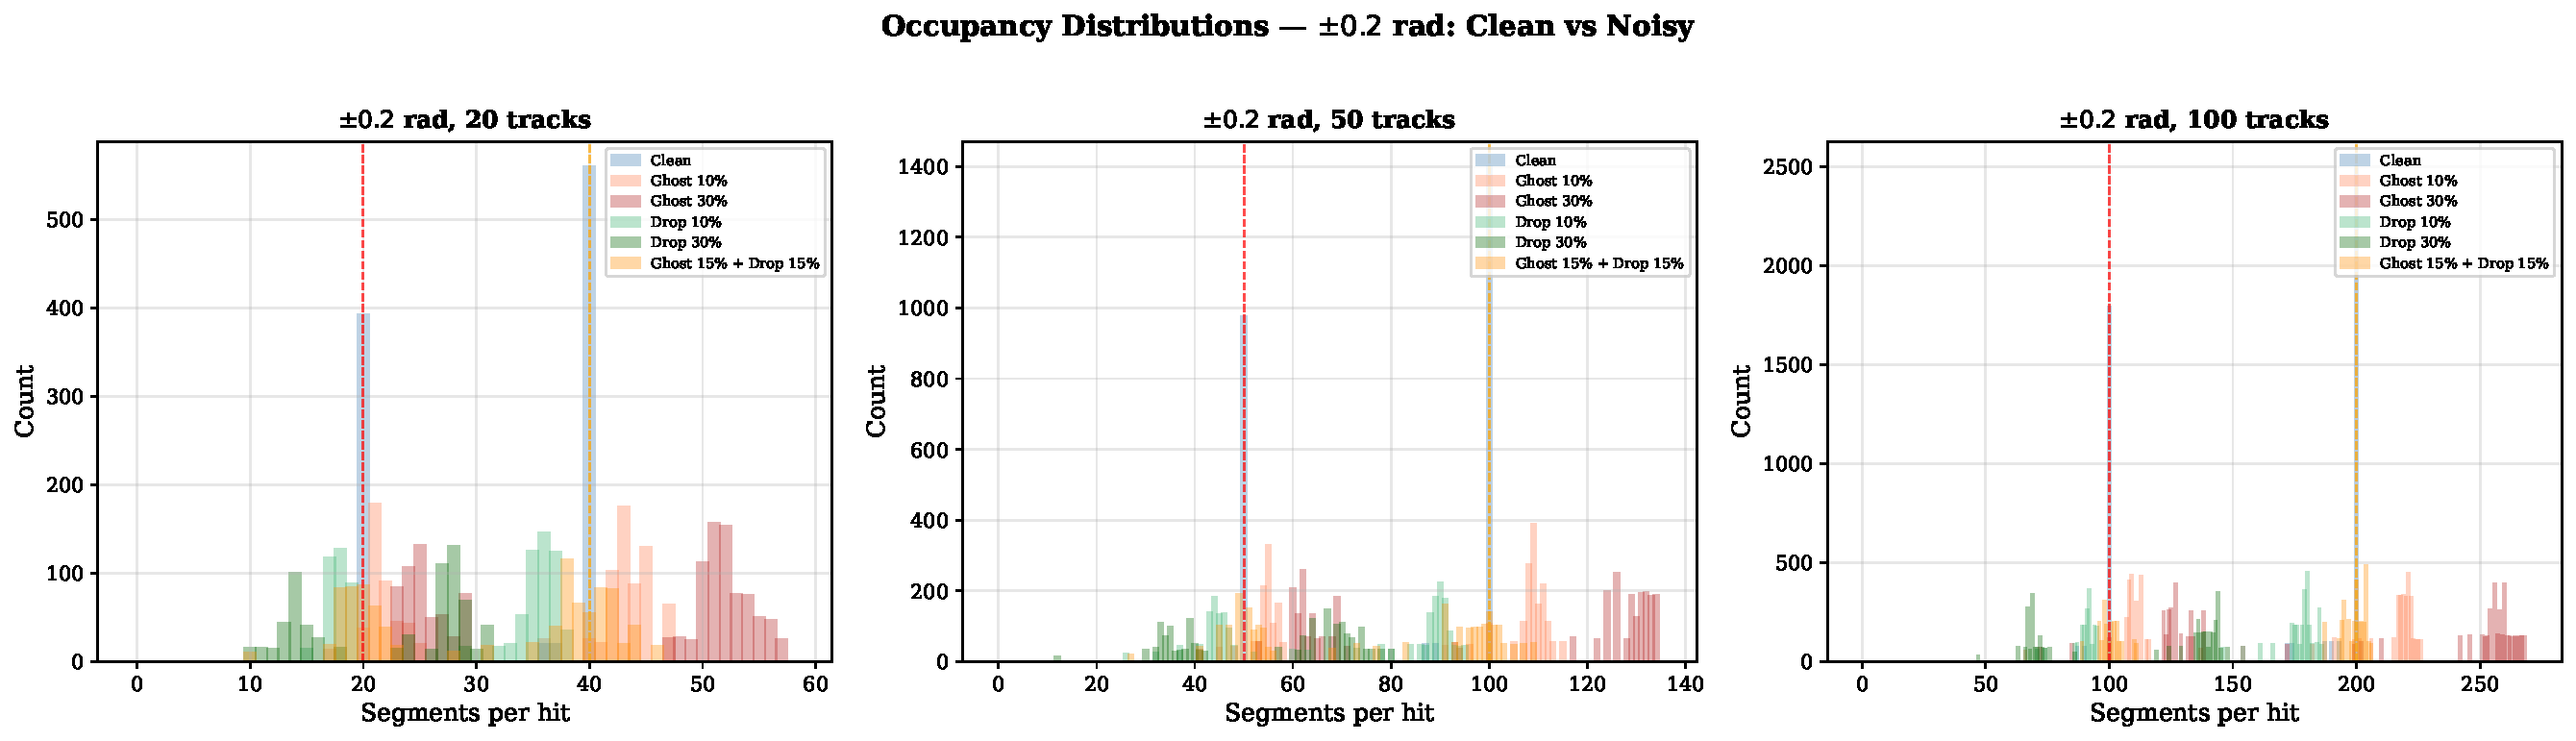
\includegraphics[width=\textwidth]{occ_hist_comparison_angle0.2}
  \caption{Occupancy distributions for $\pm 0.2$\,rad under various noise
           conditions.  Ghost hits shift mass rightward (more segments per
           hit); dropped hits reduce the peak heights.  The clean
           distribution (blue) is overlaid for reference.}
  \label{fig:occ_noisy}
\end{figure}

\subsection{Anomalous Occupancy Fraction}

Figure~\ref{fig:heatmap_anom} shows the fraction of hits whose occupancy
falls outside the expected $\{n, 2n\}$ peaks.  At the clean baseline, the
$\pm 0.2$\,rad setting already has ${\sim}4\%$ anomalous hits (from
geometric clipping); any non-zero ghost or drop rate drives this above
$70\%$.  The $\pm 0.1$\,rad control has $0\%$ anomalous hits when clean,
confirming that all anomalous counts originate from noise injection rather
than clipping.

\begin{figure}[H]
  \centering
  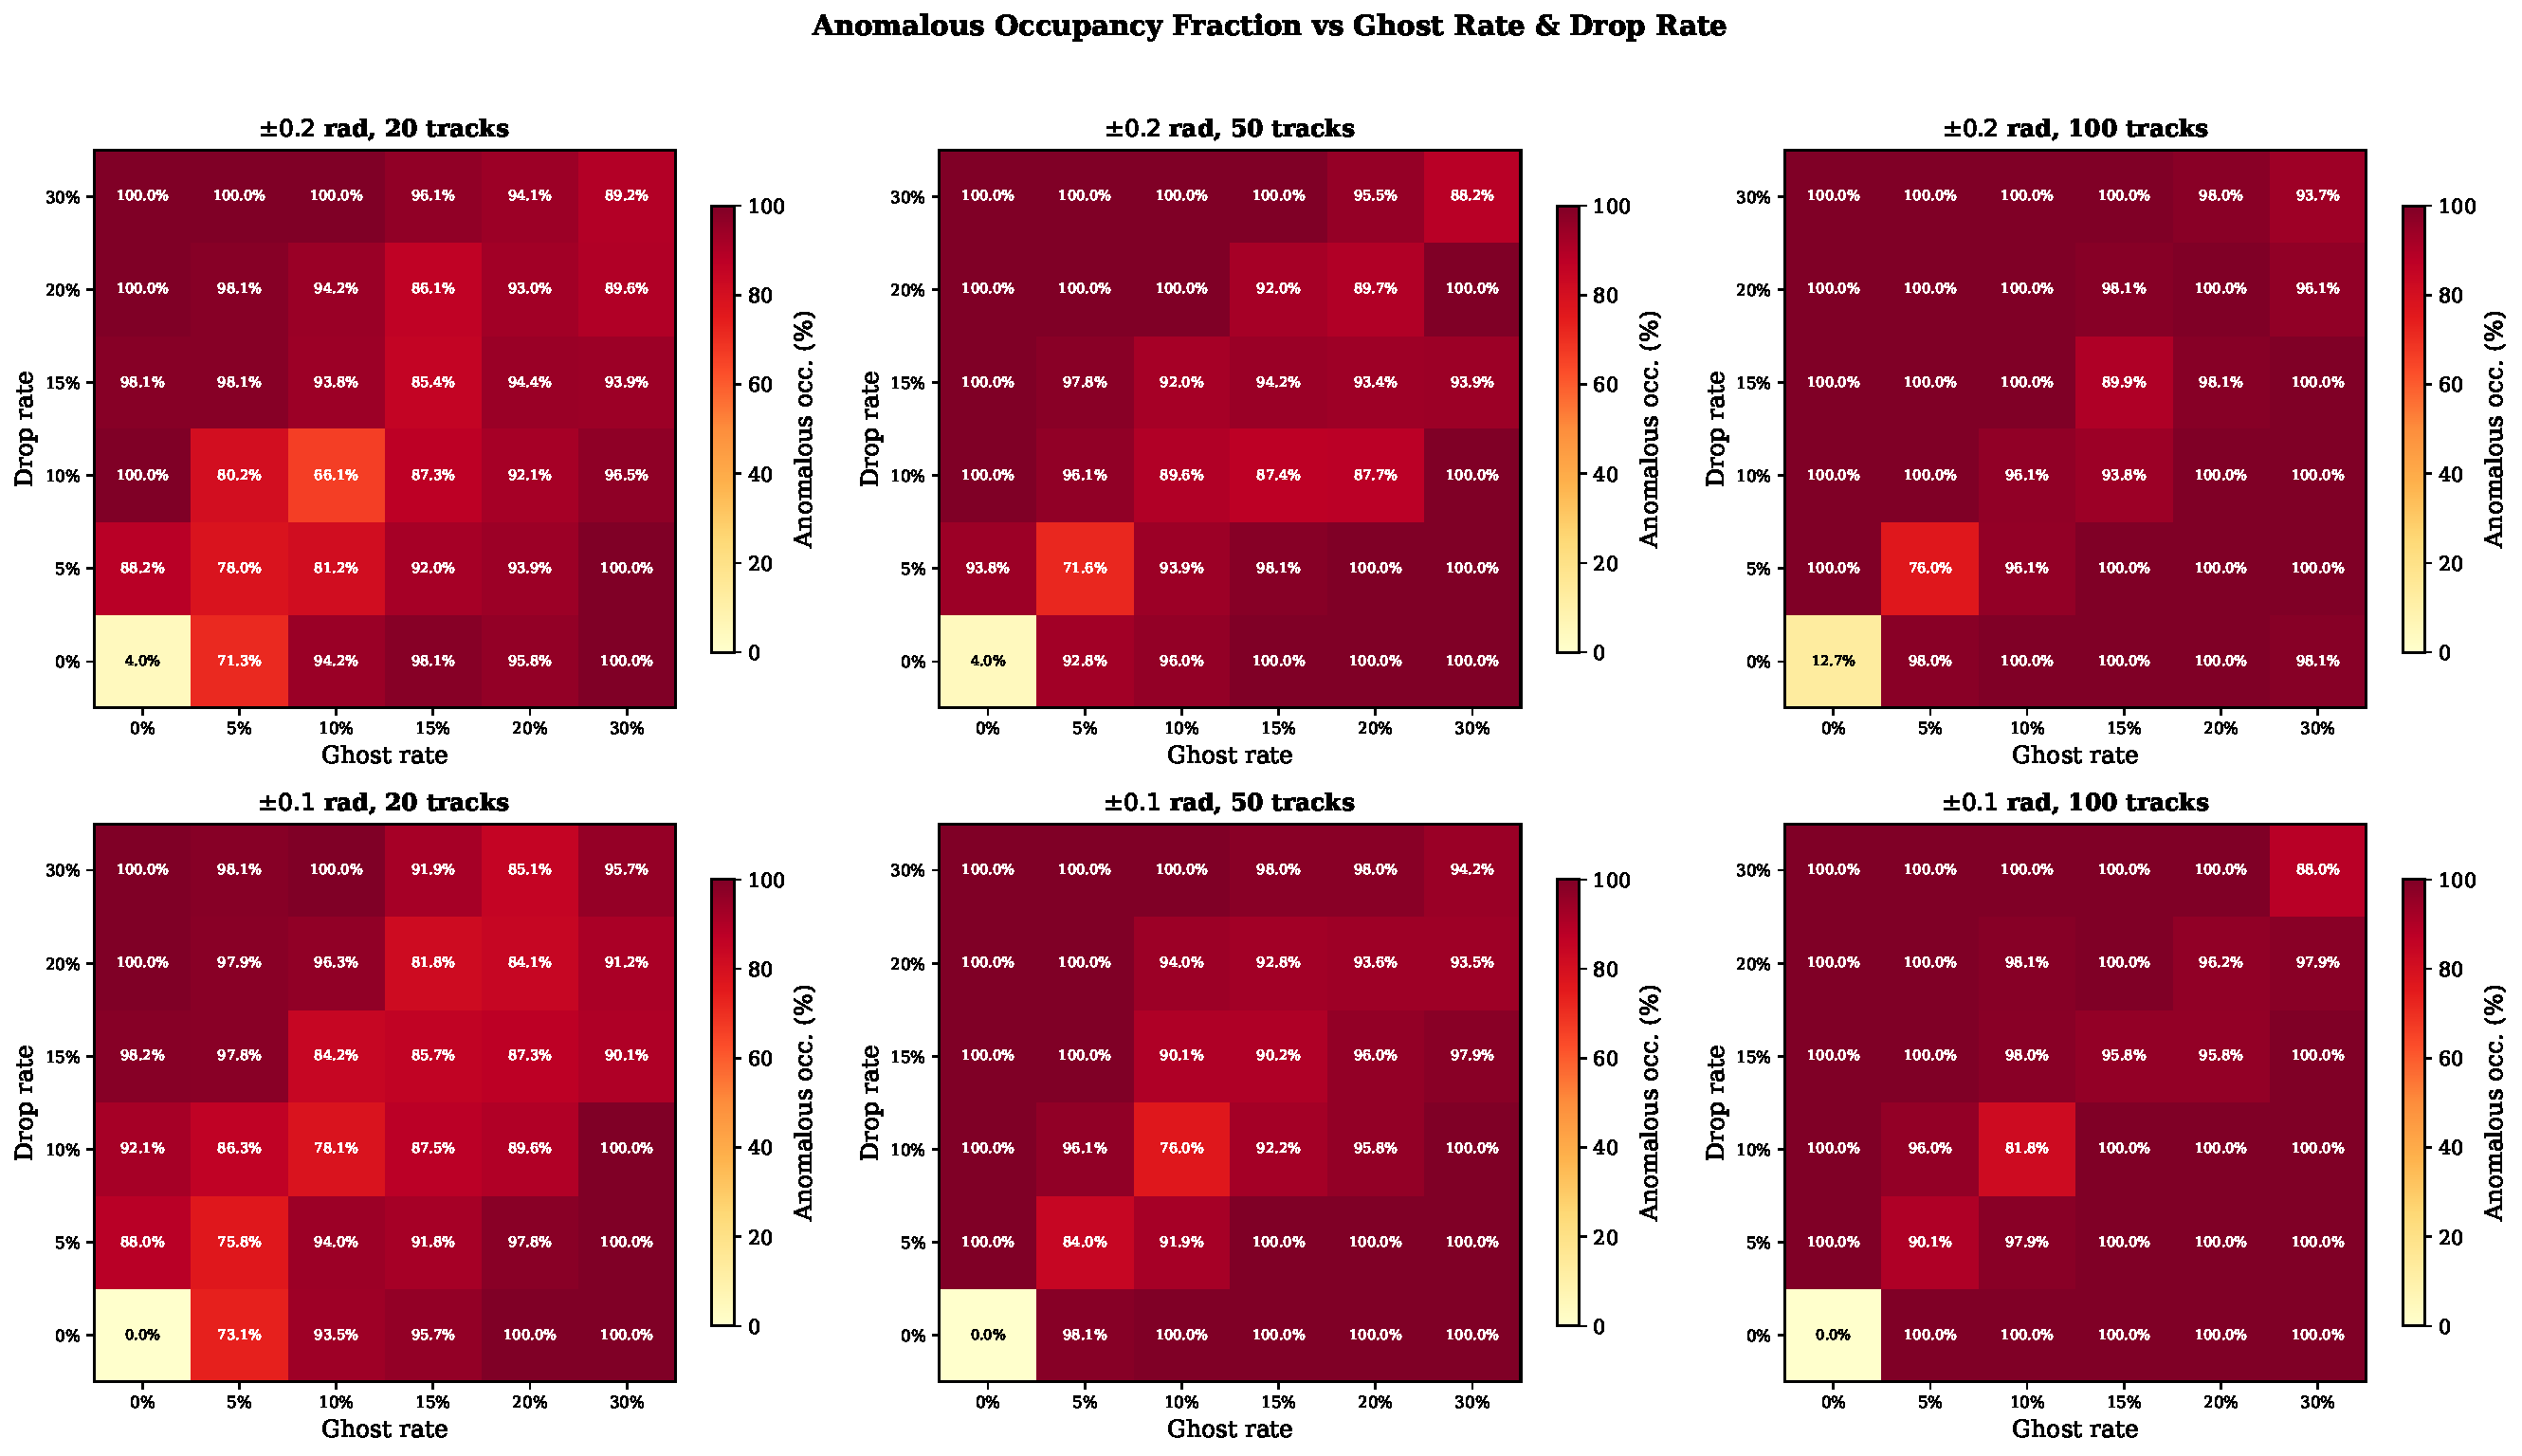
\includegraphics[width=\textwidth]{heatmap_anomalous_occ}
  \caption{Anomalous occupancy fraction as a function of ghost rate
           (columns) and drop rate (rows).  Upper panels: $\pm 0.2$\,rad;
           lower panels: $\pm 0.1$\,rad.  Columns within each row
           correspond to increasing track multiplicity.}
  \label{fig:heatmap_anom}
\end{figure}

\subsection{Reconstruction Efficiency}

Figure~\ref{fig:heatmap_eff} maps reconstruction efficiency across the
sweep grid.  Efficiency is robust to ghost hits (flat across ghost-rate
columns at fixed drop rate) but degrades sharply with the drop rate: at
$30\%$ drop, only ${\sim}30\%$ of true tracks are recovered regardless of
ghost level.  Notably, the reconstructed ghost rate and clone fraction
remain near zero across the entire sweep, indicating that the Hamiltonian
solver does not produce spurious tracks even under heavy noise.

\begin{figure}[H]
  \centering
  
\includegraphics[width=\textwidth]{heatmap_efficiency}
  \caption{Reconstruction efficiency vs ghost rate and drop rate.  Efficiency
           degrades primarily along the drop-rate axis.  Ghost hits have
           minimal impact because the $\gamma$-term suppresses false
           segments effectively.}
  \label{fig:heatmap_eff}
\end{figure}

\subsection{Segment Count Growth}

Ghost hits inflate the Hamiltonian dimension.  Figure~\ref{fig:heatmap_seg}
shows the mean number of segments.  At 100~tracks with $30\%$ ghost rate,
the segment count reaches ${\sim}65{,}000$ (compared to ${\sim}40{,}000$
clean), a $60\%$ increase.  Dropped hits reduce segment count along the
other axis, but the net effect of combined noise is dominated by ghosts.

\begin{figure}[H]
  \centering
  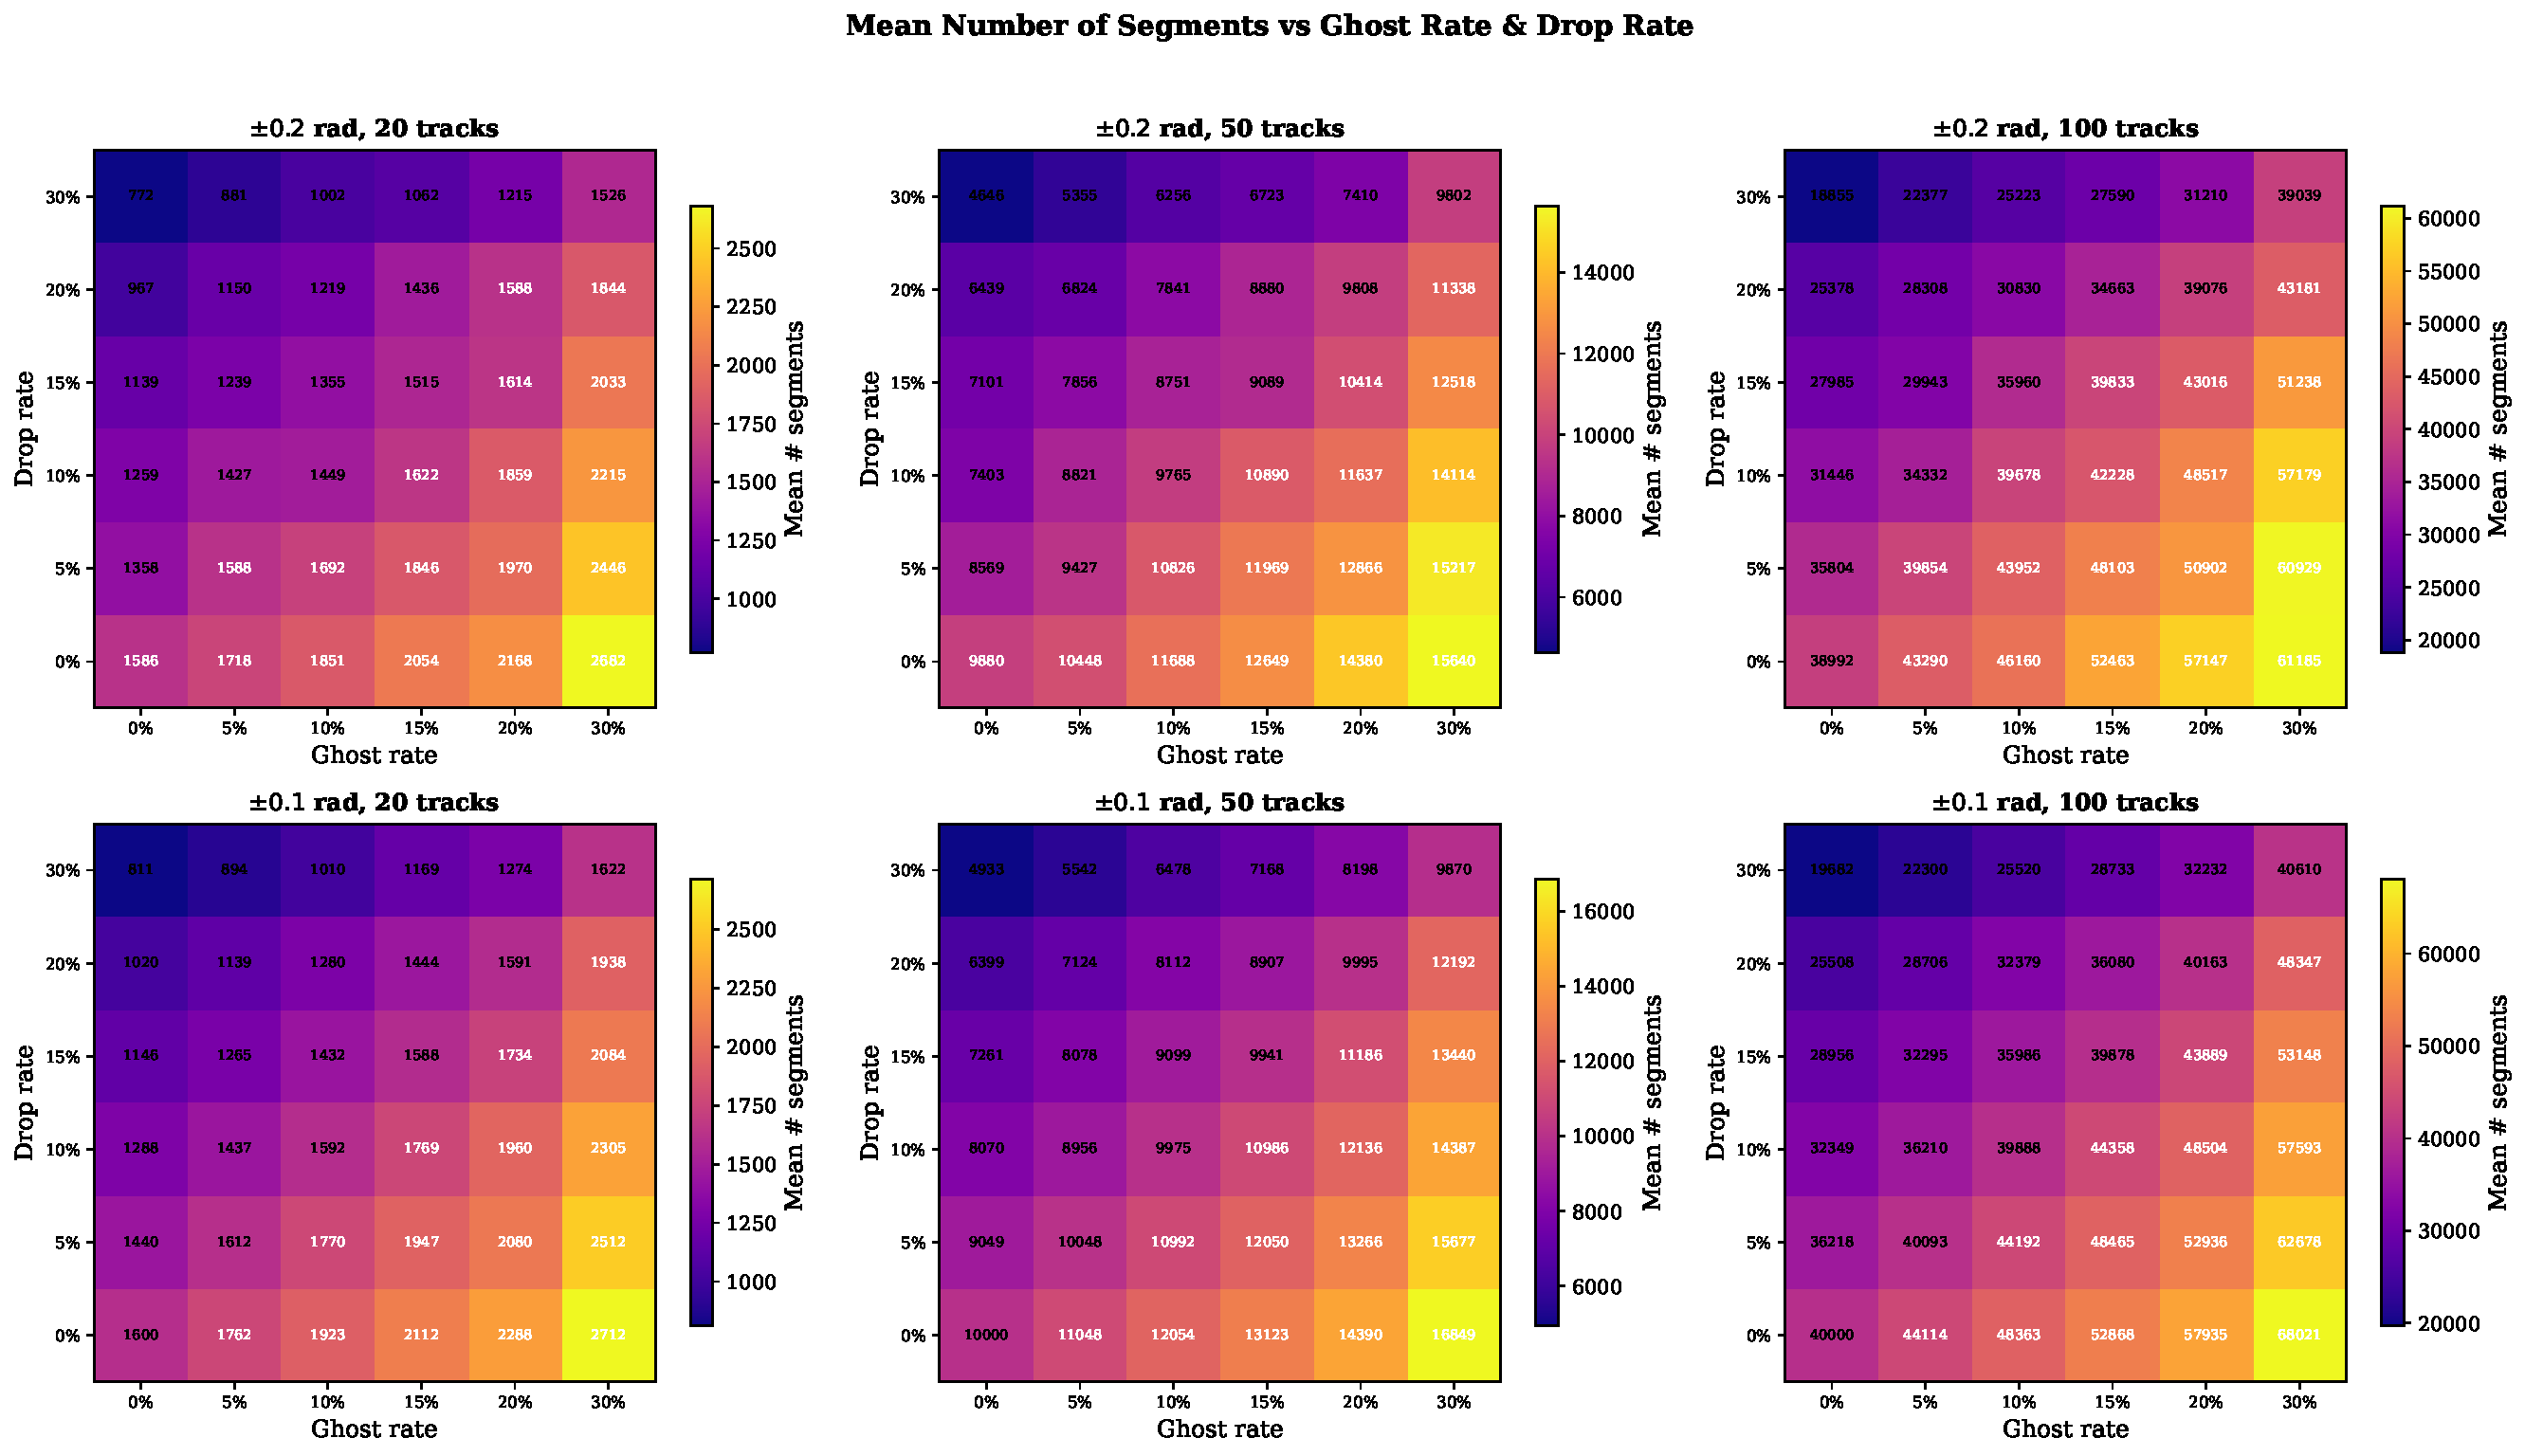
\includegraphics[width=\textwidth]{heatmap_n_segments}
  \caption{Mean number of Hamiltonian segments vs ghost and drop rate.
           Ghost hits create additional segments with all hits in adjacent
           modules, leading to super-linear growth.}
  \label{fig:heatmap_seg}
\end{figure}

\subsection{Activation Spectrum}

Figure~\ref{fig:activation} shows the mean activation of true and false
segments as a function of noise.  True-segment activations remain near
$1.09$ regardless of ghost rate, but degrade to ${\sim}0.83$ at $30\%$ drop
rate as the loss of supporting hits weakens the self-interaction term.
False-segment activations remain pinned at the baseline value
$\delta/(\delta + \gamma) \approx 0.4$ across all noise levels, confirming
that the competition mechanism suppresses false segments robustly.

\begin{figure}[H]
  \centering
  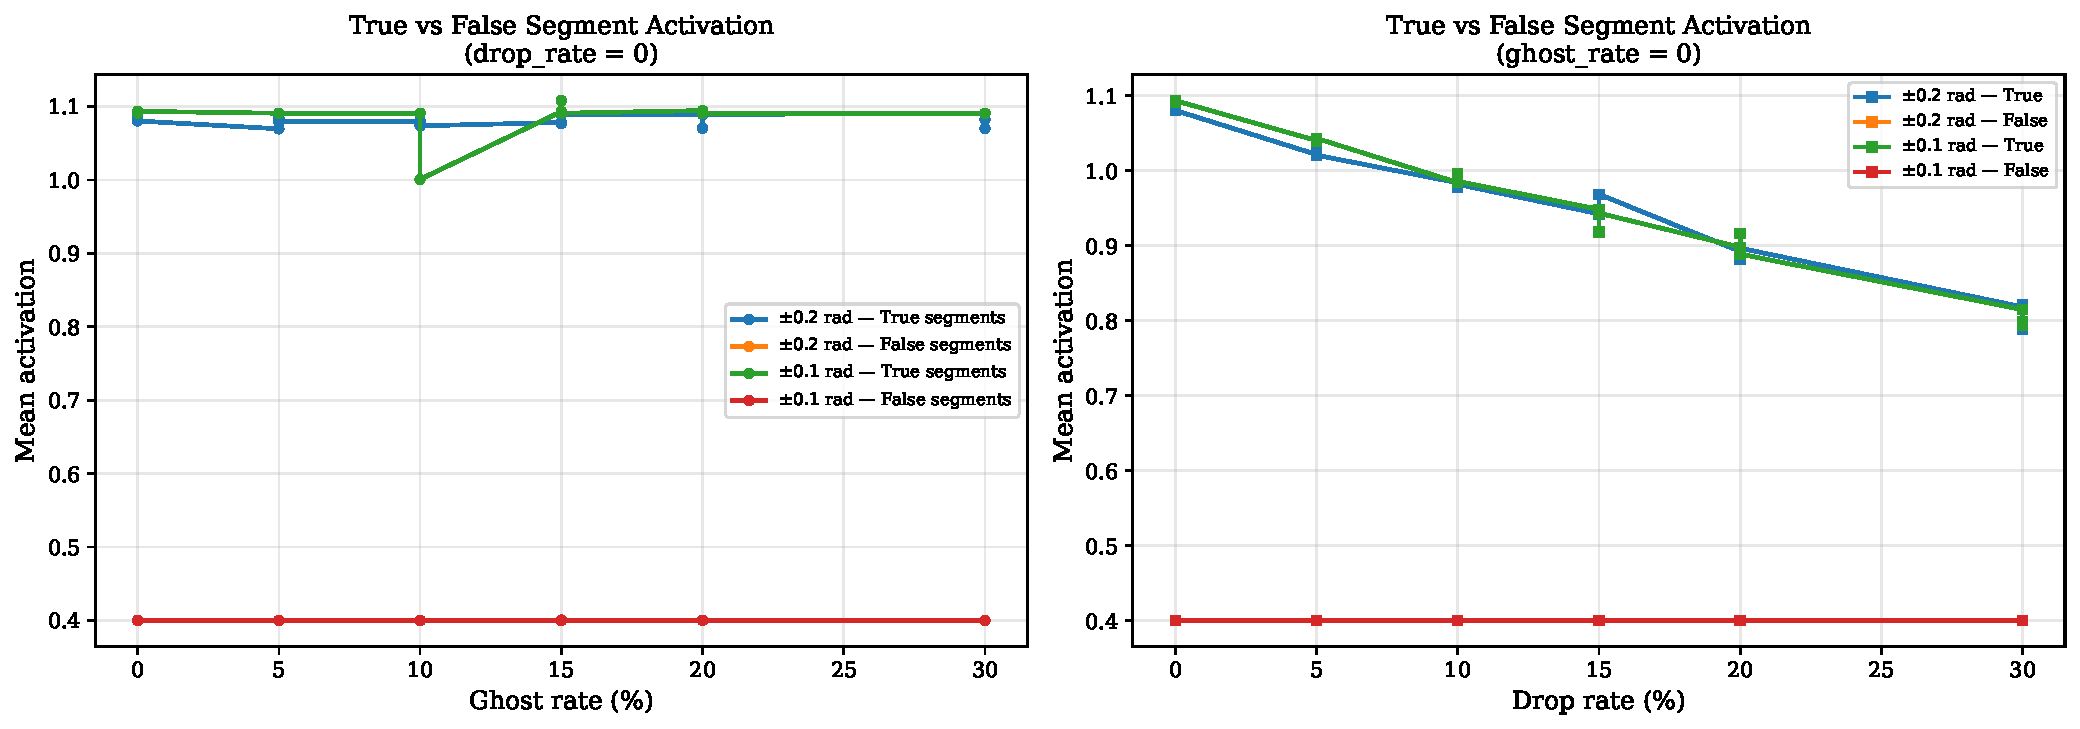
\includegraphics[width=\textwidth]{activation_spectrum}
  \caption{Mean activation of true (upper curves) and false (lower curves)
           segments.  Left: varied ghost rate at zero drop.  Right: varied
           drop rate at zero ghost.  The gap between true and false narrows
           only with increasing drop rate.}
  \label{fig:activation}
\end{figure}

% =================================================================
\section{Summary and Recommendations}
\label{sec:summary}

The ``segment grass'' occupancy sub-peaks at $\pm 0.2$\,rad are a
\textbf{geometric clipping artefact}, not a feature of the Hamiltonian or
the segment-competition mechanism.  The systematic ghost/drop-rate sweep
(Section~\ref{sec:sweep}) confirms this and reveals additional insights.
The causal chain is:

\begin{enumerate}
  \item The PV $z$-coordinate is drawn from $\mathcal{N}(0, 50^2)$\,mm,
        frequently yielding $\pvz < -15$\,mm.
  \item Tracks at the maximum angle $\phi = \pm 0.2$\,rad have slope
        $|t_x| \approx 0.203$, causing transverse displacements of up to
        $|t_x| \times (z_4 - \pvz) > 50$\,mm at the last module.
  \item These tracks miss the detector active area and produce no hit on
        the outer modules.
  \item The reduced hit count on module~$k$ lowers the occupancy of hits
        on module~$k{-}1$, creating sub-peaks in the histogram.
  \item The effect is absent at $\pm 0.1$\,rad because the corresponding
        $\zcrit$ values are $> 5\sigma$ from the PV mean.
\end{enumerate}

\noindent\textbf{Possible mitigations:}
\begin{itemize}
  \item Reduce the PV $z$ spread (e.g.\ $\sigma_z = 10$\,mm).
  \item Increase the detector half-width (e.g.\ $\halfx = 100$\,mm).
  \item Accept the effect as a realistic feature of finite detector
        acceptance and document it.
\end{itemize}

None of these sub-peaks affect the conclusions of the hit-competition
study, because the segment-competition ($\gamma$-term) mechanism operates
correctly on the segments that \emph{are} constructed.  The clipping merely
reduces the total number of segments, which is a geometric acceptance
effect independent of the Hamiltonian optimisation.

\noindent\textbf{Additional findings from the noise sweep:}
\begin{itemize}
  \item Reconstruction efficiency is robust to ghost hits but degrades
        linearly with the drop rate ($100\% \to 30\%$ at $30\%$ drop).
  \item The ghost and clone fractions in reconstructed tracks remain
        ${\sim}0\%$ even at $30\%$ ghost rate, confirming that the
        $\gamma$-term successfully suppresses false segments.
  \item Ghost hits inflate the Hamiltonian by up to $60\%$ (at 100~tracks,
        $30\%$ ghost), increasing computational cost without improving
        physics reach.
  \item True-segment activations degrade only with the drop rate (from
        $1.09$ to $0.83$ at $30\%$ drop), while false-segment activations
        remain suppressed at the baseline $\approx 0.4$.
\end{itemize}

\end{document}
